\documentclass{article}
\usepackage[utf8]{inputenc}

% Page setup
\usepackage[a4paper,landscape,margin=2cm]{geometry}
\usepackage{amsmath}

% Typography
\usepackage[scaled]{helvet}
\let\familydefault\sfdefault

\usepackage[usenames,svgnames]{xcolor}
\usepackage{tikz,pgfplots}
\usetikzlibrary{positioning,arrows,intersections}

\definecolor{colordict}     {RGB}{143,232,186}
\definecolor{colortext}     {RGB}{29 ,29 ,27 }
\definecolor{colordelta}    {RGB}{199,212,104}

\begin{document}
\pagestyle{empty}
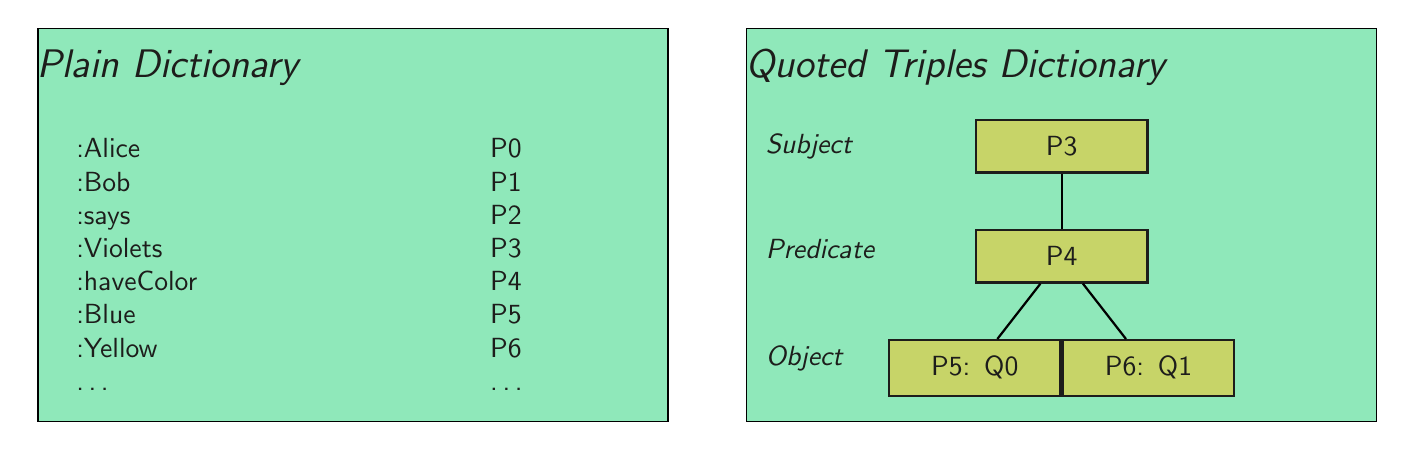
\begin{tikzpicture}[
    node distance = 2em, auto,
    font={\Large\itshape},
    title/.style={text=colortext,font={\Large\itshape}},
    code/.style={text=colortext,font={}},
    base/.style={text=colortext,font={},inner sep=6pt,align=center,rectangle},
    treenode/.style={base,thick,draw=colortext,text width=5em},
]

    \draw[fill=colordict] (0,0) rectangle (8,5);
    \node[title,text width=20em] at (3.5,4.5) {Plain Dictionary};
    \node[code,text width=20em] at (4,2) {:Alice\\
    :Bob\\
    :says\\
    :Violets\\
    :haveColor\\
    :Blue\\
    :Yellow\\
    \ldots};
    \node[code,text width=10em] at (7.5,2) {P0\\
    P1\\
    P2\\
    P3\\
    P4\\
    P5\\
    P6\\
    \ldots};
    
    \draw[fill=colordict] (9,0) rectangle (17,5);
    \node[title,text width=20em] at (12.5,4.5) {Quoted Triples Dictionary};
    \node[treenode,fill=colordelta] at (13,3.5) (ts1)        {P3};
    \node[treenode,fill=colordelta,below=of ts1.south] (tp1) {P4};
    \node[treenode,fill=colordelta,below=of tp1.south west] (to1) {P5: Q0};
    \node[treenode,fill=colordelta,below=of tp1.south east] (to2) {P6: Q1};
    \draw[-,thick](tp1) -- (ts1);
    \draw[-,thick](to1) -- (tp1);
    \draw[-,thick](to2) -- (tp1);
    \node[code,text width=10em,font={\itshape}] at (11,3.5) {Subject};
    \node[code,text width=10em,font={\itshape}] at (11,2.2) {Predicate};
    \node[code,text width=10em,font={\itshape}] at (11,0.8) {Object};

\end{tikzpicture}
\end{document}
